\documentclass[aspectratio=169]{beamer}

% ---------- ENCODING & FONTS (prevents Unicode dash/quotes issues) ----------
\usepackage[utf8]{inputenc}
\usepackage[T1]{fontenc}

% ---------- THEME & LOOK ----------
\usetheme{Madrid}
\usecolortheme{seahorse}
\usefonttheme{professionalfonts}
\setbeamertemplate{navigation symbols}{}
\setbeamercovered{transparent}
\setbeamertemplate{itemize items}[circle]
\setbeamertemplate{enumerate items}[default]
\setlength{\parskip}{0.25em}

% ---------- COLORS ----------
\usepackage{xcolor}
\definecolor{accent}{RGB}{0,92,184}
\definecolor{soft}{RGB}{233,244,255}
\setbeamercolor{structure}{fg=accent}
\setbeamercolor{title}{fg=white,bg=accent}
\setbeamercolor{frametitle}{fg=accent}
\setbeamercolor{block title}{bg=accent!12,fg=accent}
\setbeamercolor{block body}{bg=soft}

% ---------- PACKAGES ----------
\usepackage{booktabs}
\usepackage{amsmath, amssymb}
\usepackage{array}
\usepackage{hyperref}
\hypersetup{colorlinks=true,linkcolor=accent,urlcolor=accent}

% ---------- SAFE FALLBACK FOR TRANSITIONS ----------
\makeatletter
\@ifundefined{transfade}{\newcommand{\transfade}[1][]{}}{}
\makeatother

% ---------- PLACEHOLDER BOX (compile-safe; no images required) ----------
\newcommand{\placeholderbox}[2][0.82\linewidth]{%
  \begin{center}
    \fbox{\begin{minipage}[c][0.46\textheight][c]{#1}
      \centering \vspace{0.25em}
      \textbf{#2}\\[0.6em]
      \emph{Insert figure/diagram here later.}
    \end{minipage}}
  \end{center}
}

% ---------- TITLE ----------
\title{\textbf{The Economics of Immigration  \vspace{.5cm}\\  }}
\subtitle{ {\large ECON 300 - Labour Economics}}
%\institute{UNBC}
\author{Muhebullah Karimzada}

\date{Winter 2026}


\begin{document}

% ============================================================
% TITLE
% ============================================================
\begin{frame}[plain]
  \titlepage
\end{frame}

% ============================================================
\section{Learning Objectives \& Questions}
% ============================================================

\begin{frame}{Learning Objectives}
\transfade
\begin{itemize}[<+->]
  \item Describe the profile of immigrants to Canada: how many arrive, origins, destinations.
  \item Explain Canada’s point system and how it shapes admissions.
  \item Use supply and demand to evaluate immigration’s effects on wages and employment.
  \item Define earnings assimilation and explain cross-section vs.\ cohort pitfalls.
  \item Sketch a simple migration model and decision rule for moving countries.
\end{itemize}
\end{frame}

\begin{frame}{Main Questions}
\transfade
\begin{itemize}[<+->]
  \item How have immigration patterns to Canada evolved over 60 years?
  \item What is the point system and how does it affect who immigrates?
  \item Do higher inflows put downward pressure on wages or raise unemployment?
  \item How fast do immigrants’ earnings catch up to native-born Canadians?
  \item Are immigrants a net drain on public finances?
\end{itemize}
\end{frame}

% ============================================================
\section{Profile of Immigration to Canada}
% ============================================================

\begin{frame}{Trends and Source Regions}
\transfade
\begin{itemize}[<+->]
  \item Until mid-1980s, immigration levels fluctuated widely.
  \item \(\sim\)200k/year to late-1990s; rising thereafter to 270k+ by 2015.
  \item Per-capita inflows slightly lower than peak historical episodes.
  \item Source regions changed dramatically over time.
\end{itemize}
\end{frame}

\begin{frame}{Figure 11.1 -- Immigration to Canada by Source Region, 1955--2019 }
\centering
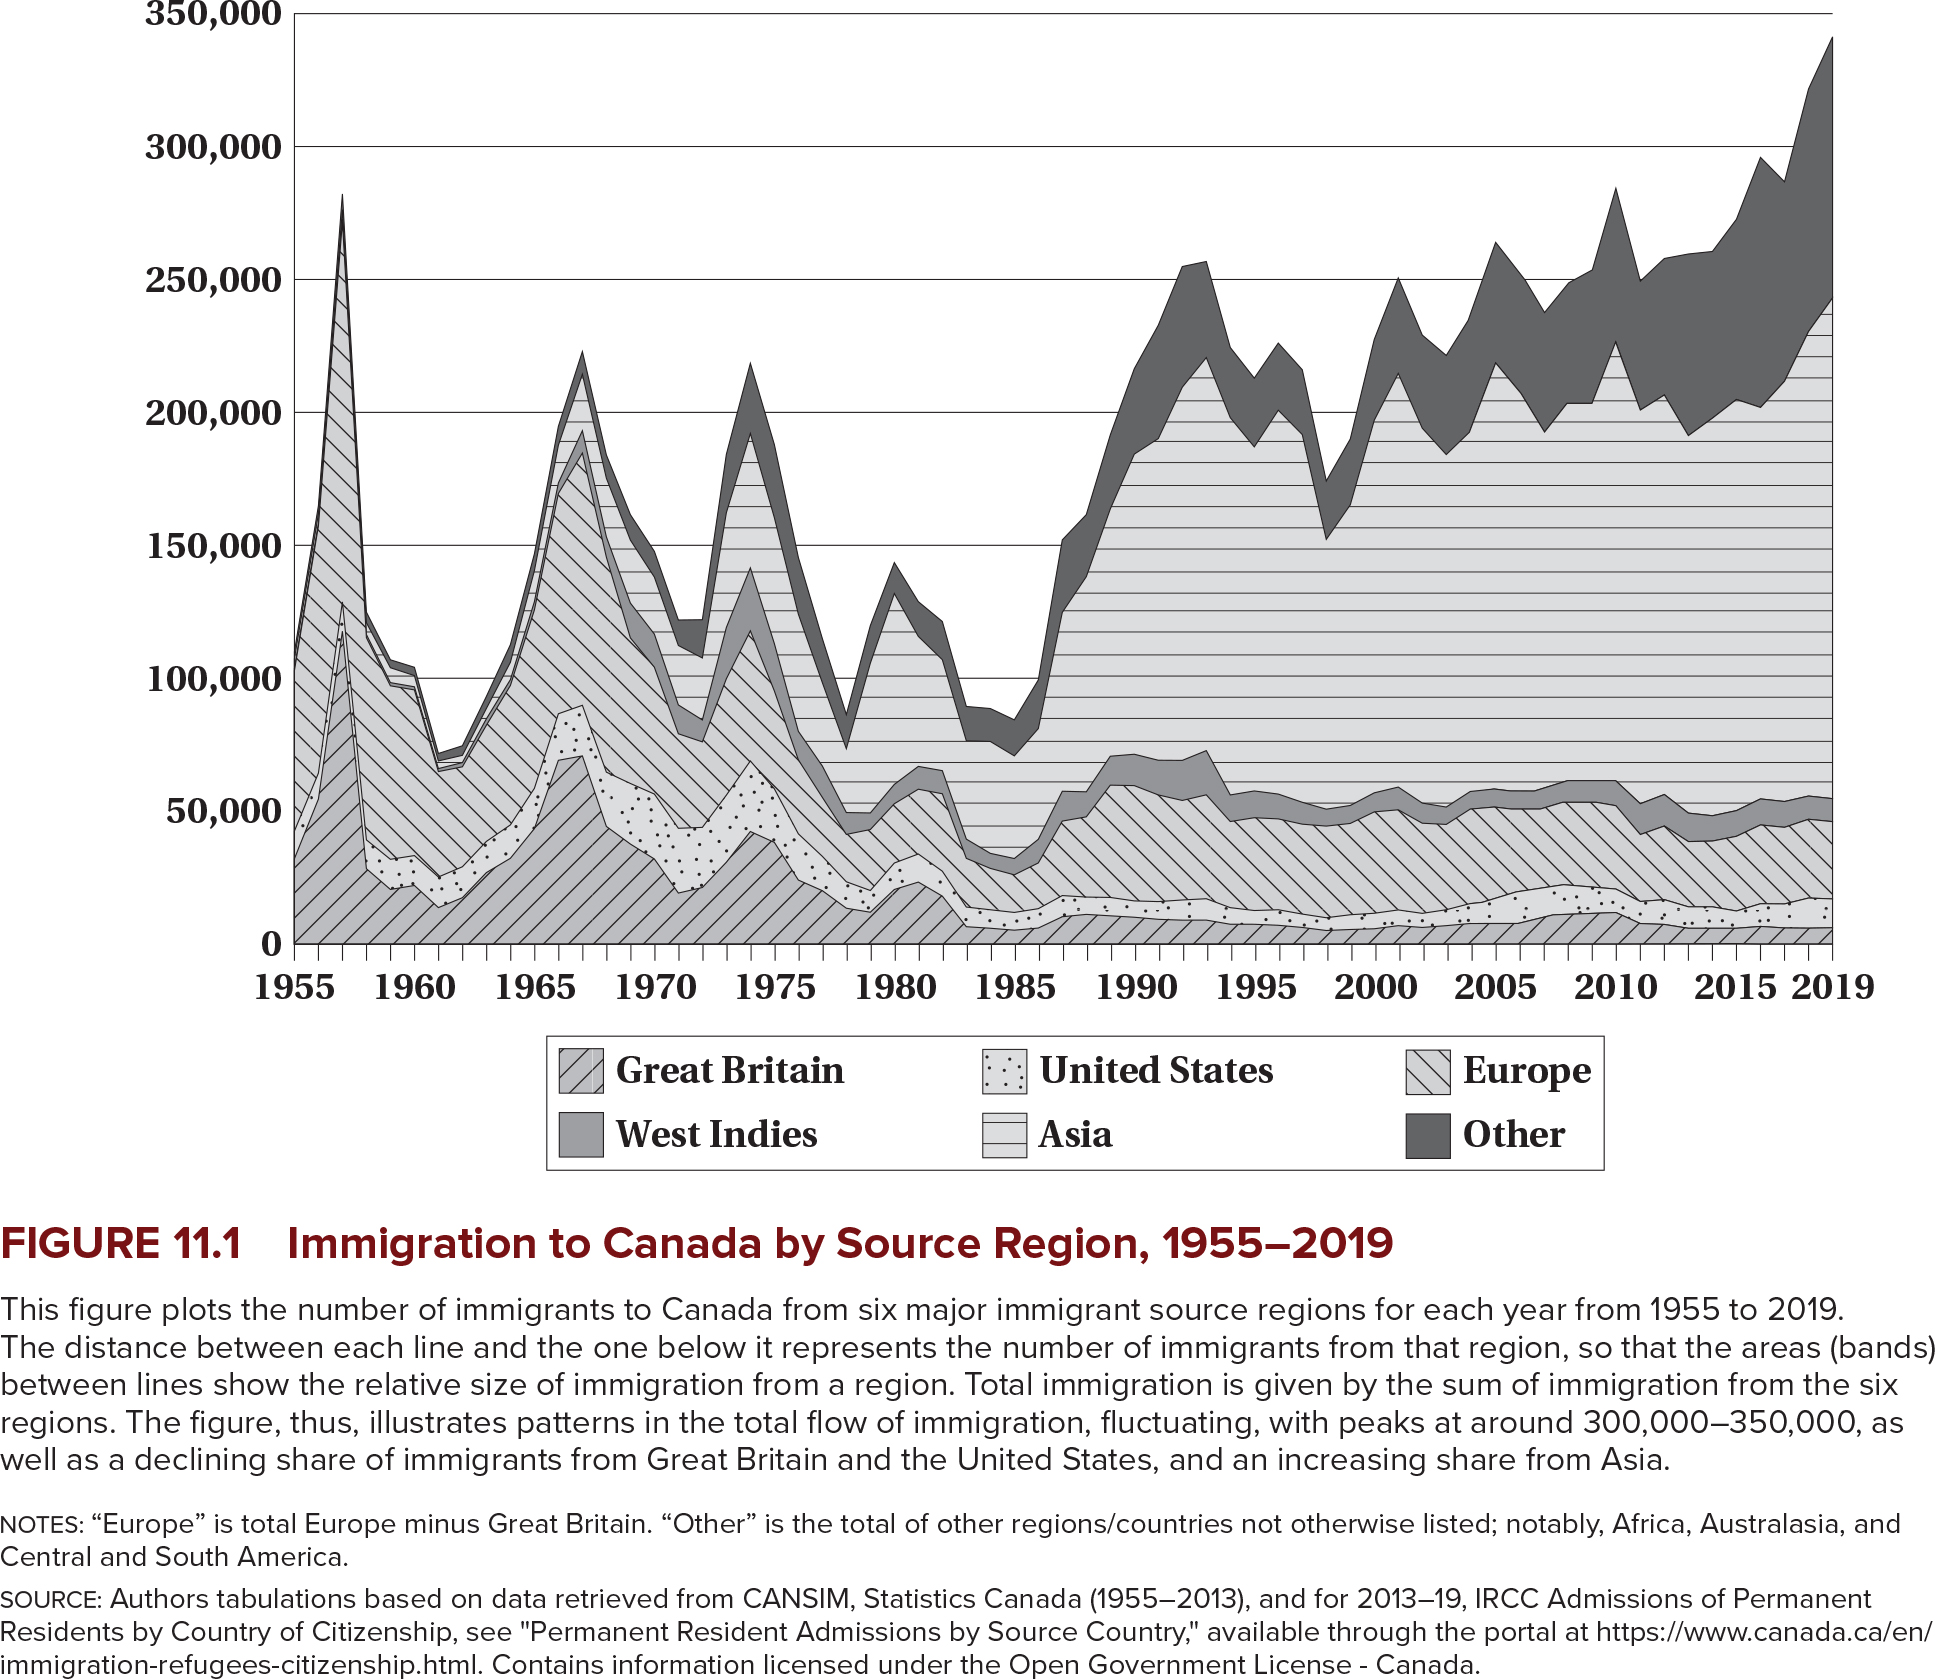
\includegraphics[width=0.8\linewidth]{ben54842_1101}
\end{frame}

\begin{frame}{Table 11.1 -- Top Ten Immigrant Source Countries, 2005 and 2019}
\centering
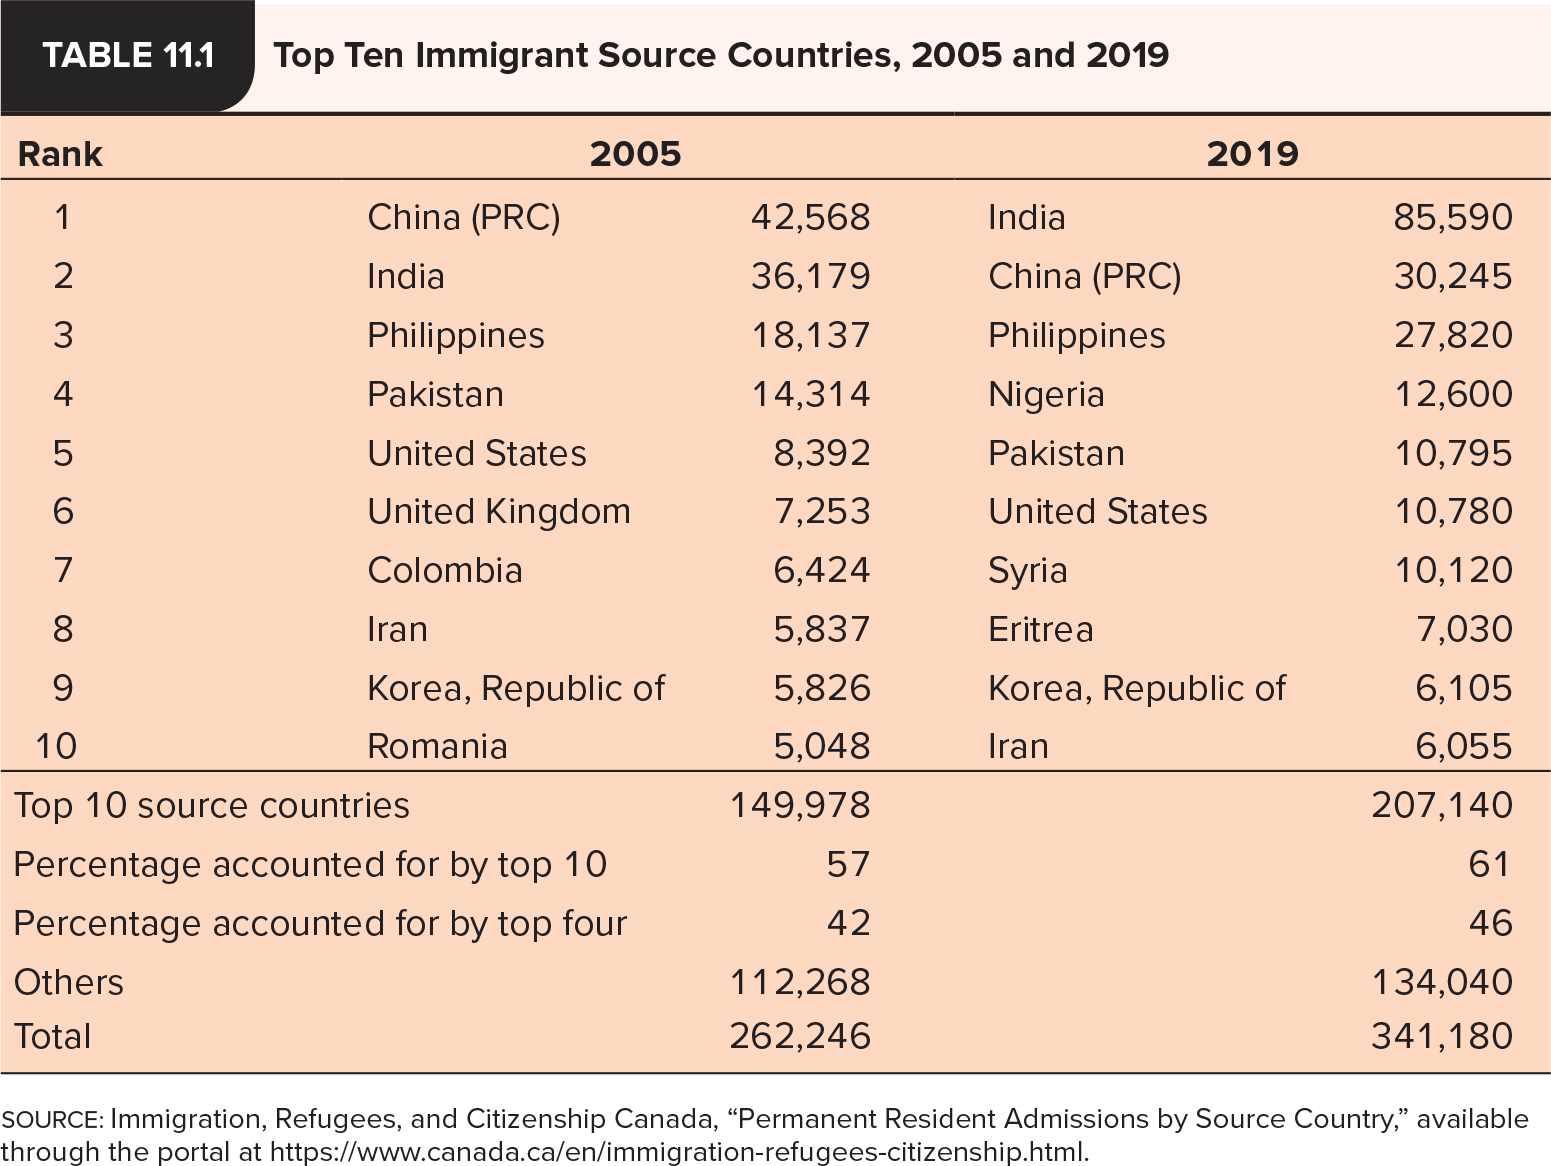
\includegraphics[width=0.7\linewidth]{ben54842_tb1101}
\end{frame}

\begin{frame}{Figure 11.2 -- Immigrant Concentration by CMA, 2006 and 2016 }
\centering
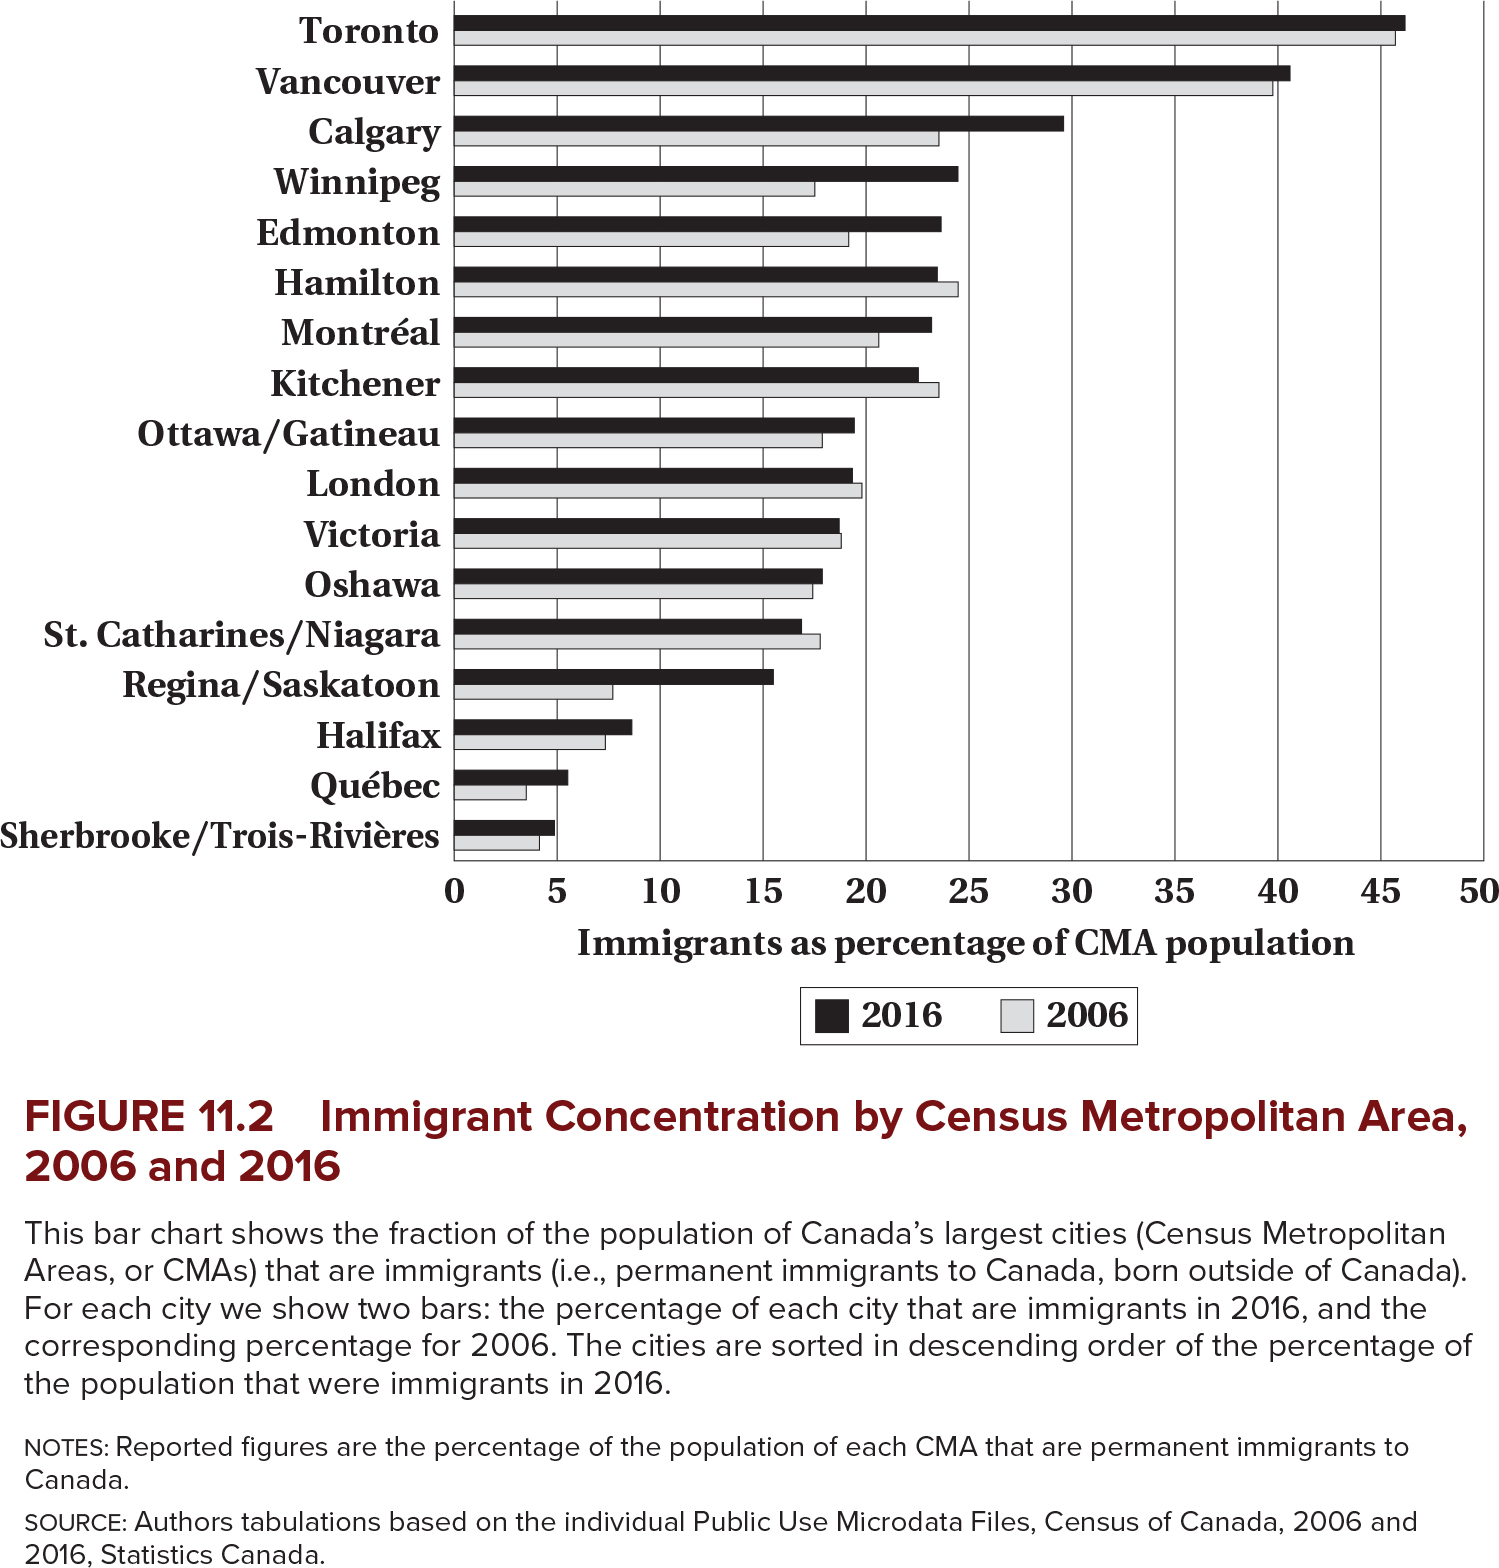
\includegraphics[width=0.68\linewidth]{ben54842_1102}
\end{frame}

% ============================================================
\section{Policy Environment \& Point System}
% ============================================================

\begin{frame}{Two Policy Levers}
\transfade
\begin{itemize}[<+->]
  \item \textbf{How many} immigrants to admit.
  \item \textbf{Who} is admitted (selection rules).
\end{itemize}
\end{frame}

\begin{frame}{Objectives of Immigration Policy}
\transfade
\begin{itemize}[<+->]
  \item Maximize national welfare.
  \item Alleviate skill shortages and support growth.
  \item Family reunification.
  \item Humanitarian protection.
\end{itemize}
\end{frame}

\begin{frame}{Two Admission Classes}
\transfade
\begin{itemize}[<+->]
  \item \textbf{Assessed}: Independent immigrants evaluated on expected labour-market success; point system.
  \item \textbf{Non-assessed}: Family and refugee classes.
\end{itemize}
\end{frame}

\begin{frame}{Canada’s Immigration Point System (circa 2016)}
\transfade
\begin{itemize}[<+->]
  \item \textbf{Work experience}: \(\ge\)1 year recent full-time in a broadly skilled occupation.
  \item \textbf{Language}: Minimum score on sanctioned language test.
  \item \textbf{Minimum funds}: Sufficient start-up funds on arrival.
  \item \textbf{Minimum score}: At least 67/100 across six criteria:
    \begin{itemize}[<+->]
      \item Education (25), Official language (28), Work experience (15),
      \item Age (10), Arranged employment (10), Adaptability (10).
    \end{itemize}
\end{itemize}
\end{frame}

\begin{frame}{Figure 11.3 -- Immigration to Canada by Class, 1966--2019 }
\centering
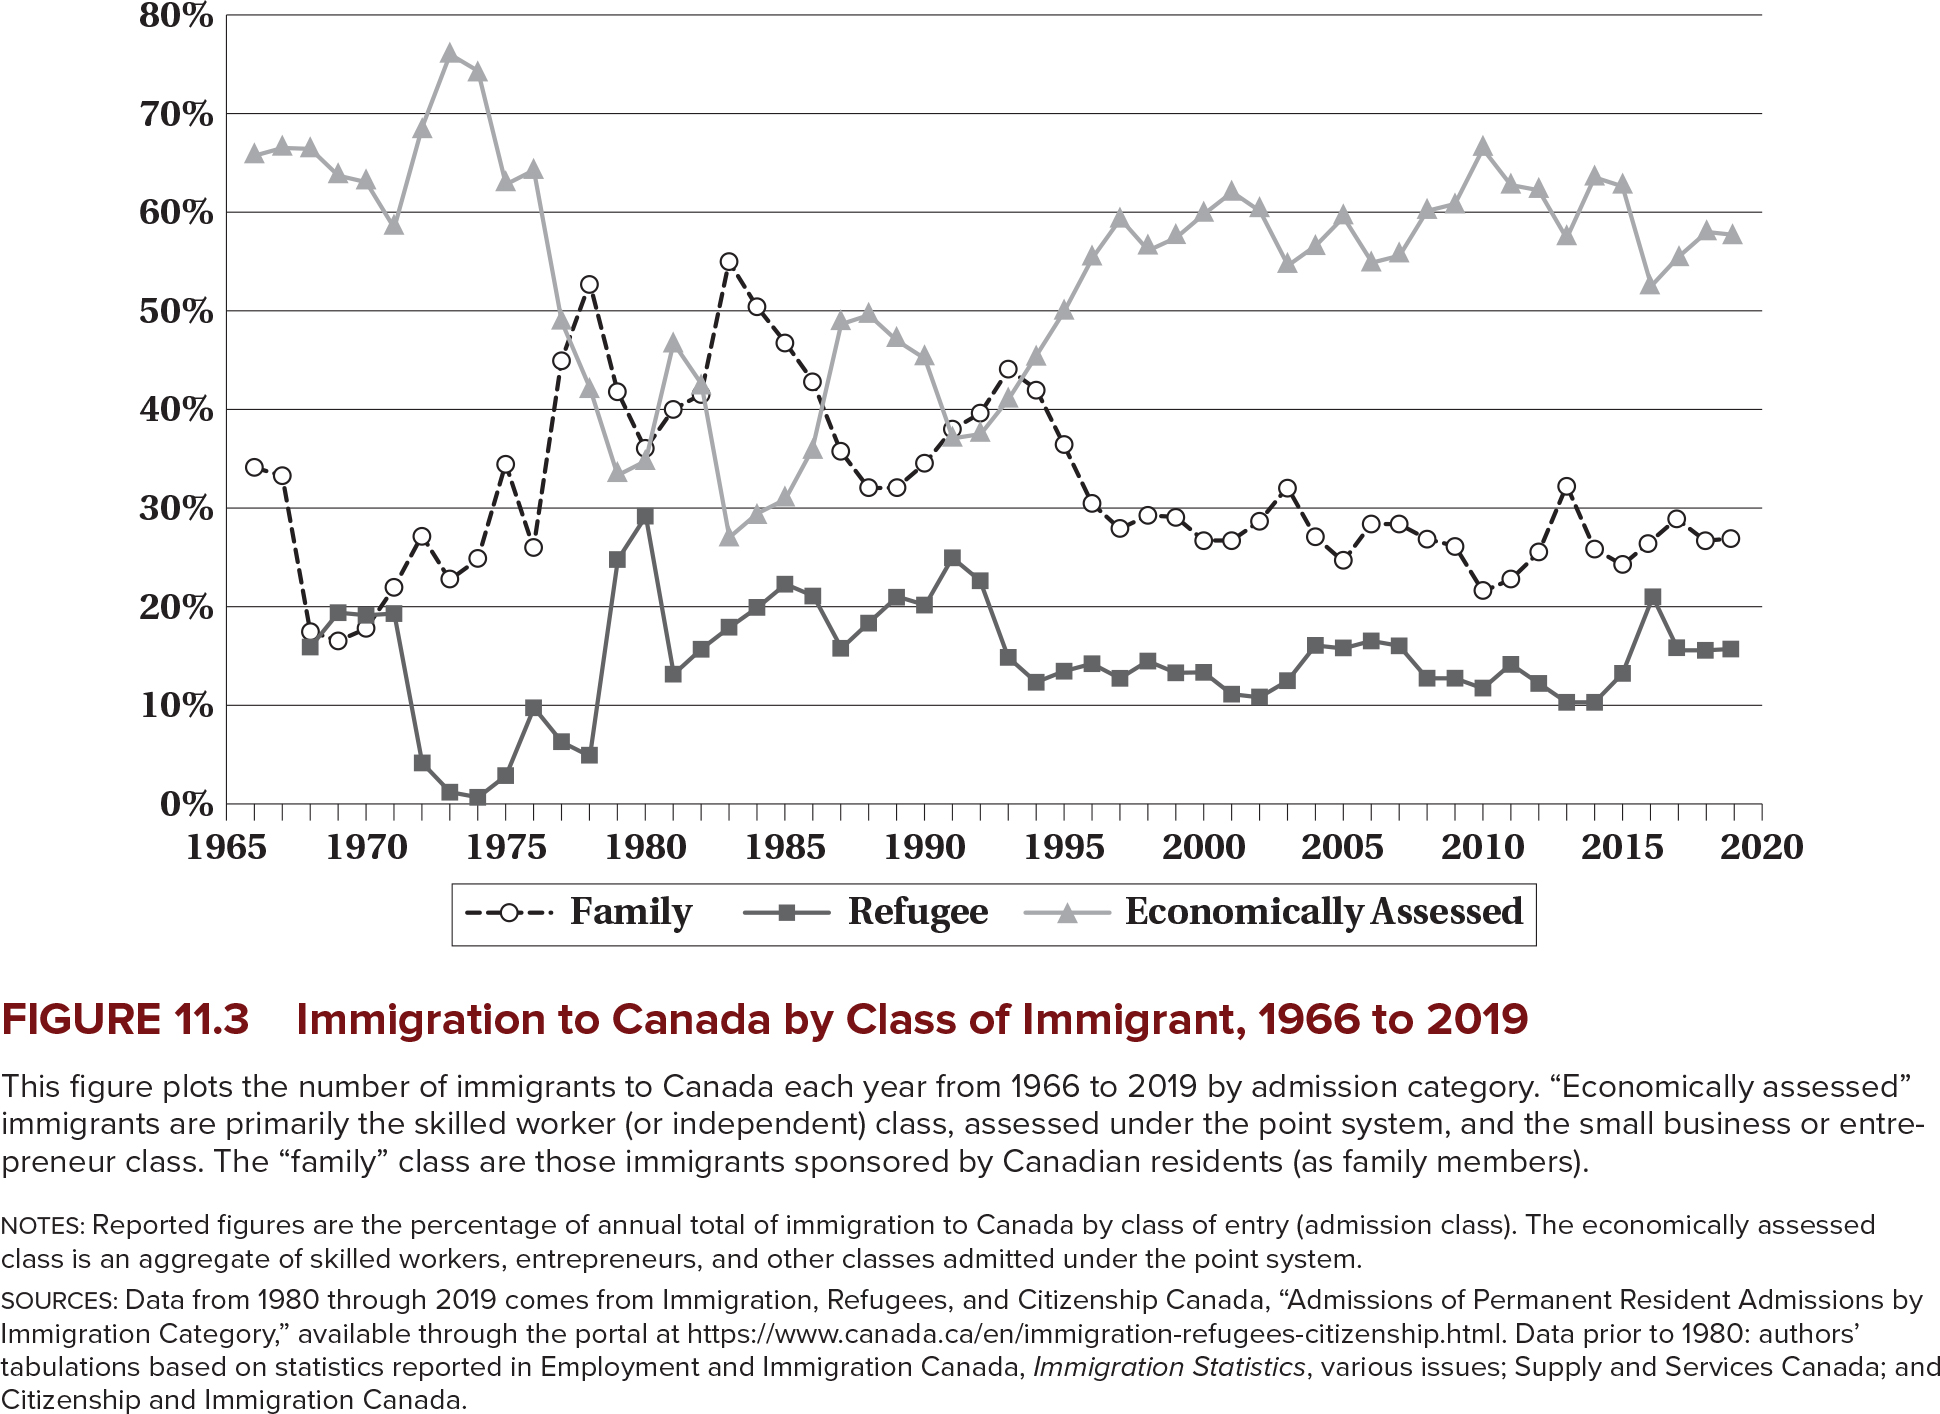
\includegraphics[width=0.96\linewidth]{ben54842_1103}
\end{frame}

% ============================================================
\section{Labour-Market Impact Framework}
% ============================================================

\begin{frame}{Supply--Demand Logic}
\transfade
\begin{itemize}[<+->]
  \item Immigration shifts \textbf{labour supply} right in receiving markets.
  \item Wage/employment effects depend on \textbf{elasticities}, capital adjustment, and skill mix.
  \item Complementarity vs.\ substitutability across skills is crucial for incidence.
\end{itemize}
\end{frame}

\begin{frame}{Figure 11.4 -- Impact of Immigration on Employment and Wages }
\centering
\vspace{.37cm}
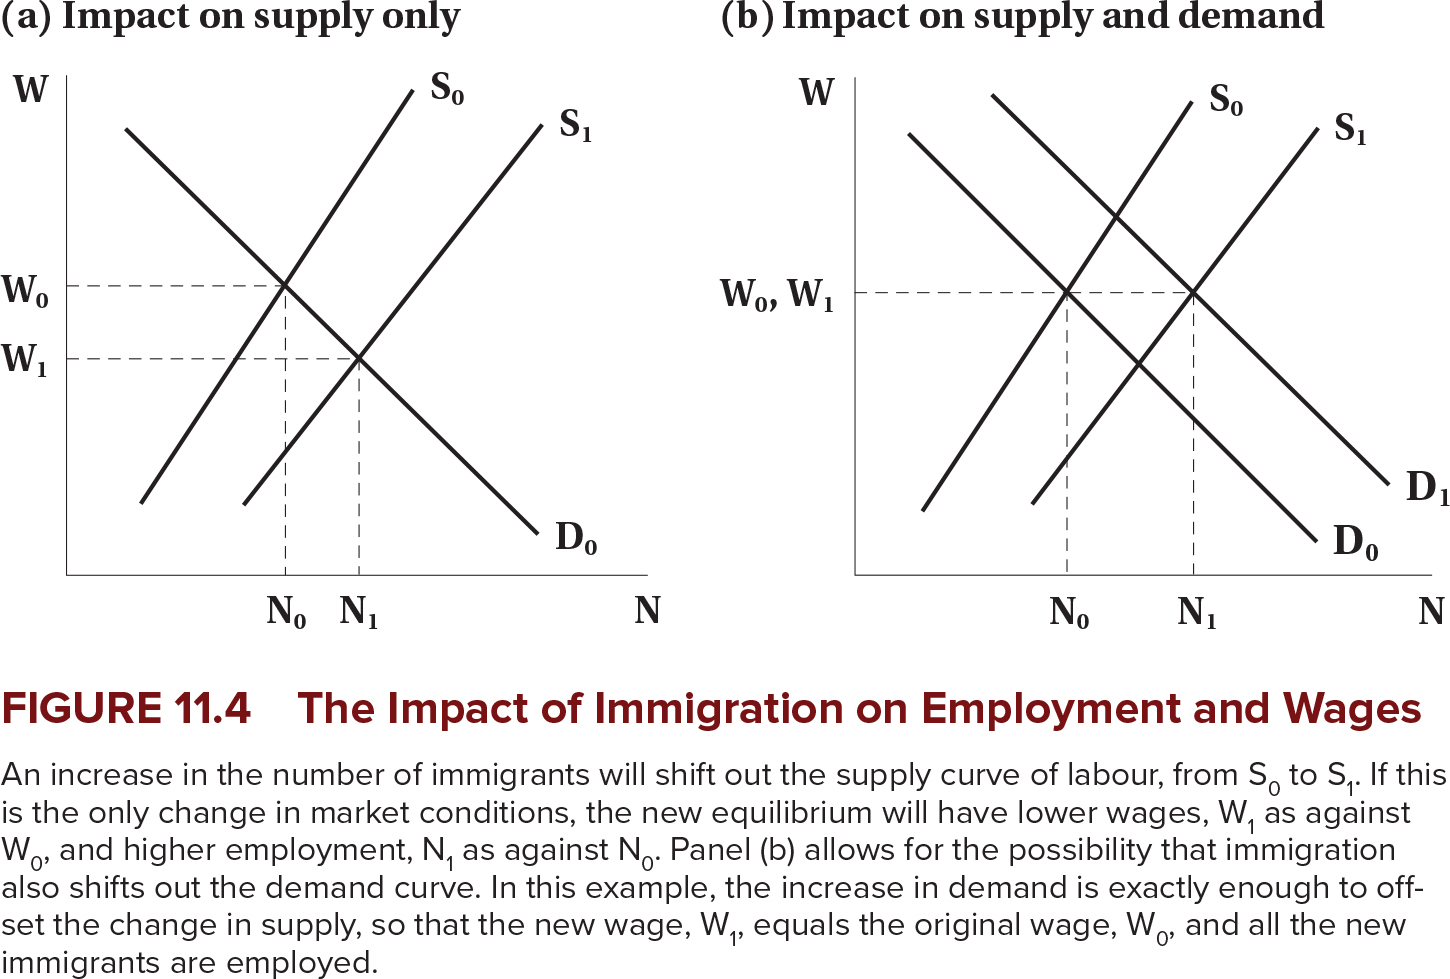
\includegraphics[width=.99\linewidth]{ben54842_1104}
\end{frame}

\begin{frame}{Estimating the Effects: Strategies}
\transfade
\begin{itemize}[<+->]
  \item \textbf{Counterfactual problem}: Where would wages be without immigration?
  \item \textbf{Cross-city variation}: Compare high- vs.\ low-immigration cities.
  \item \textbf{Natural experiments}: Exploit sudden inflow shocks.
  \item Combined approaches to strengthen identification.
\end{itemize}
\end{frame}

\begin{frame}{Findings from Empirical Research}
\transfade
\begin{itemize}[<+->]
  \item Hard to find strong adverse average effects on the native-born.
  \item Strong \textbf{skill dimension}: outcomes vary by education/experience groups.
\end{itemize}
\end{frame}

% ============================================================
\section{Economic Assimilation}
% ============================================================

\begin{frame}{Assimilation Concepts}
\transfade
\begin{itemize}[<+->]
  \item Immigrants may start with lower hours or earnings (entry effect).
  \item Earnings typically rise with time in country (experience, language, credentials).
\end{itemize}
\end{frame}

\begin{frame}{Figure 11.5 -- Hypothetical Assimilation Profile (Age 20)}
\centering
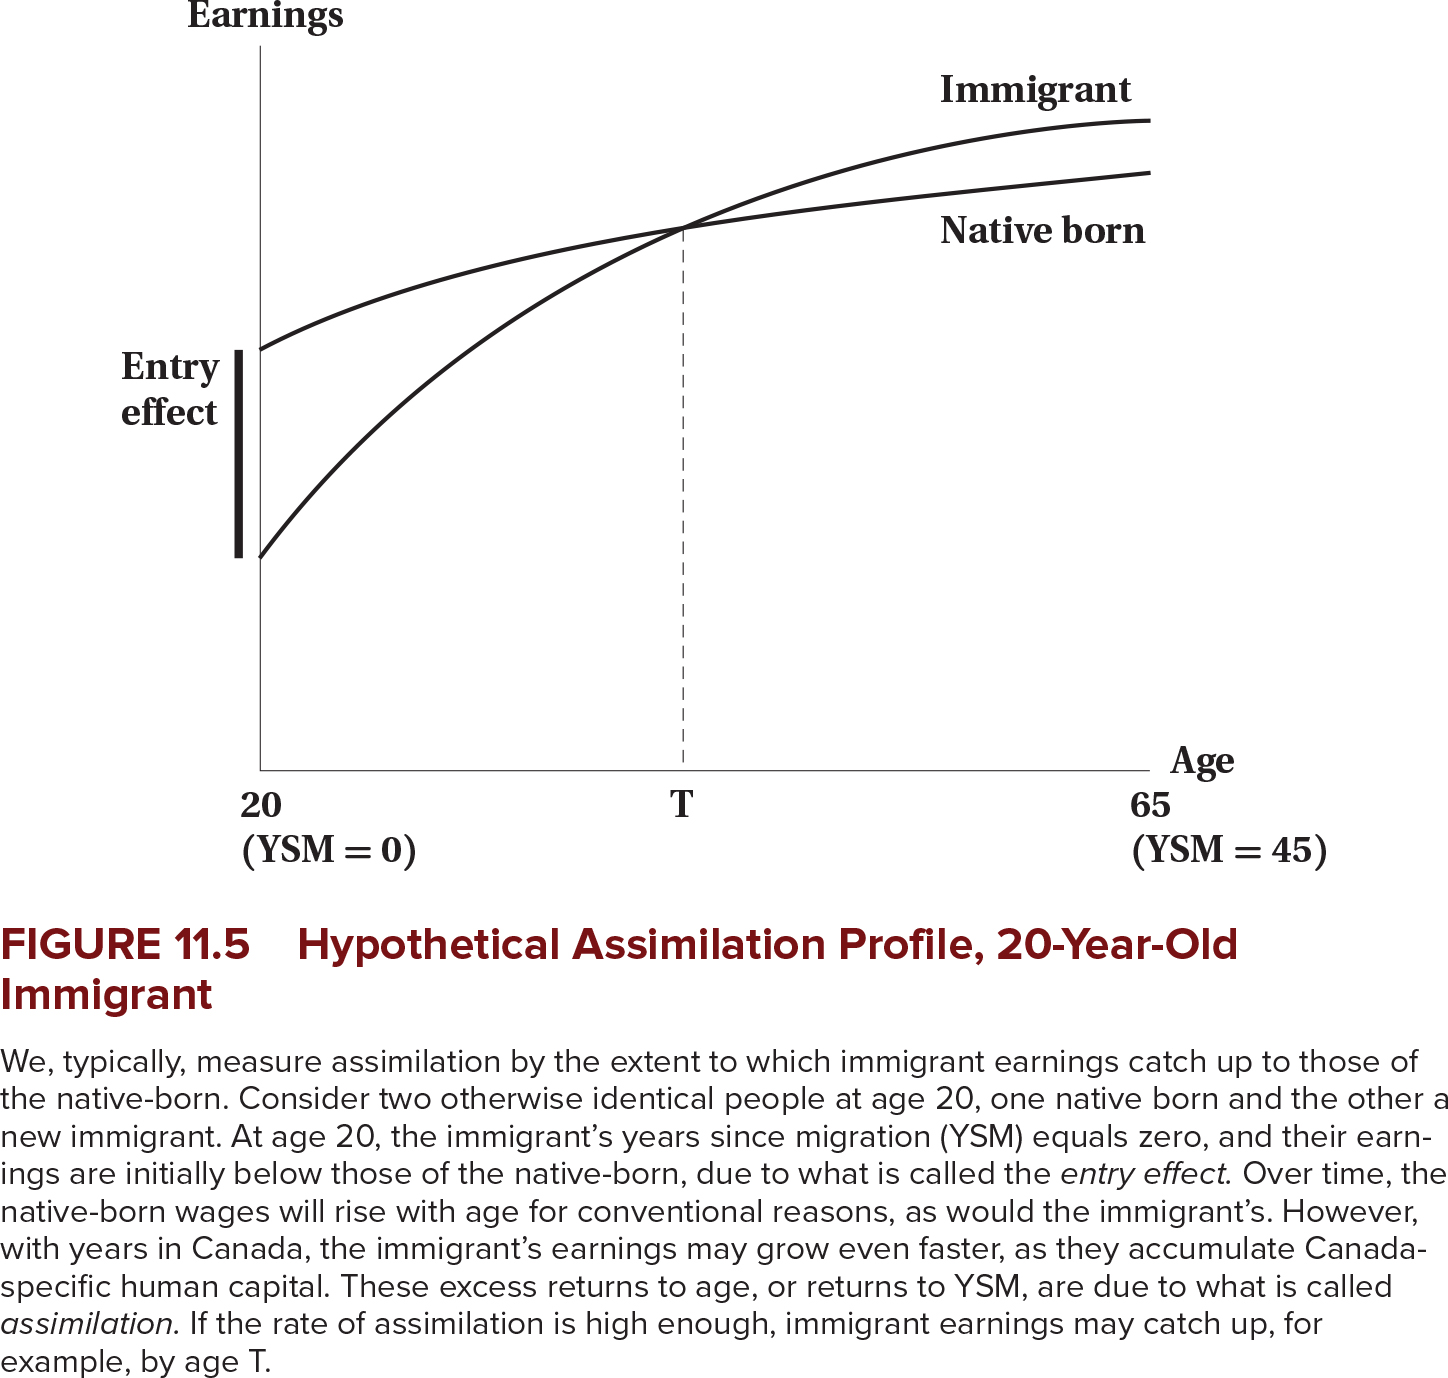
\includegraphics[width=0.78\linewidth]{ben54842_1105}
\end{frame}

\begin{frame}{Measuring Assimilation Properly}
\transfade
\begin{itemize}[<+->]
  \item Cross-sections confound \textbf{cohort} differences with \textbf{time-since-arrival}.
  \item Quasi-panels track cohorts to separate cohort vs.\ assimilation effects.
\end{itemize}
\end{frame}

\begin{frame}{Figure 11.6 -- Disentangling Cohort vs.\ Assimilation Effects }
\centering
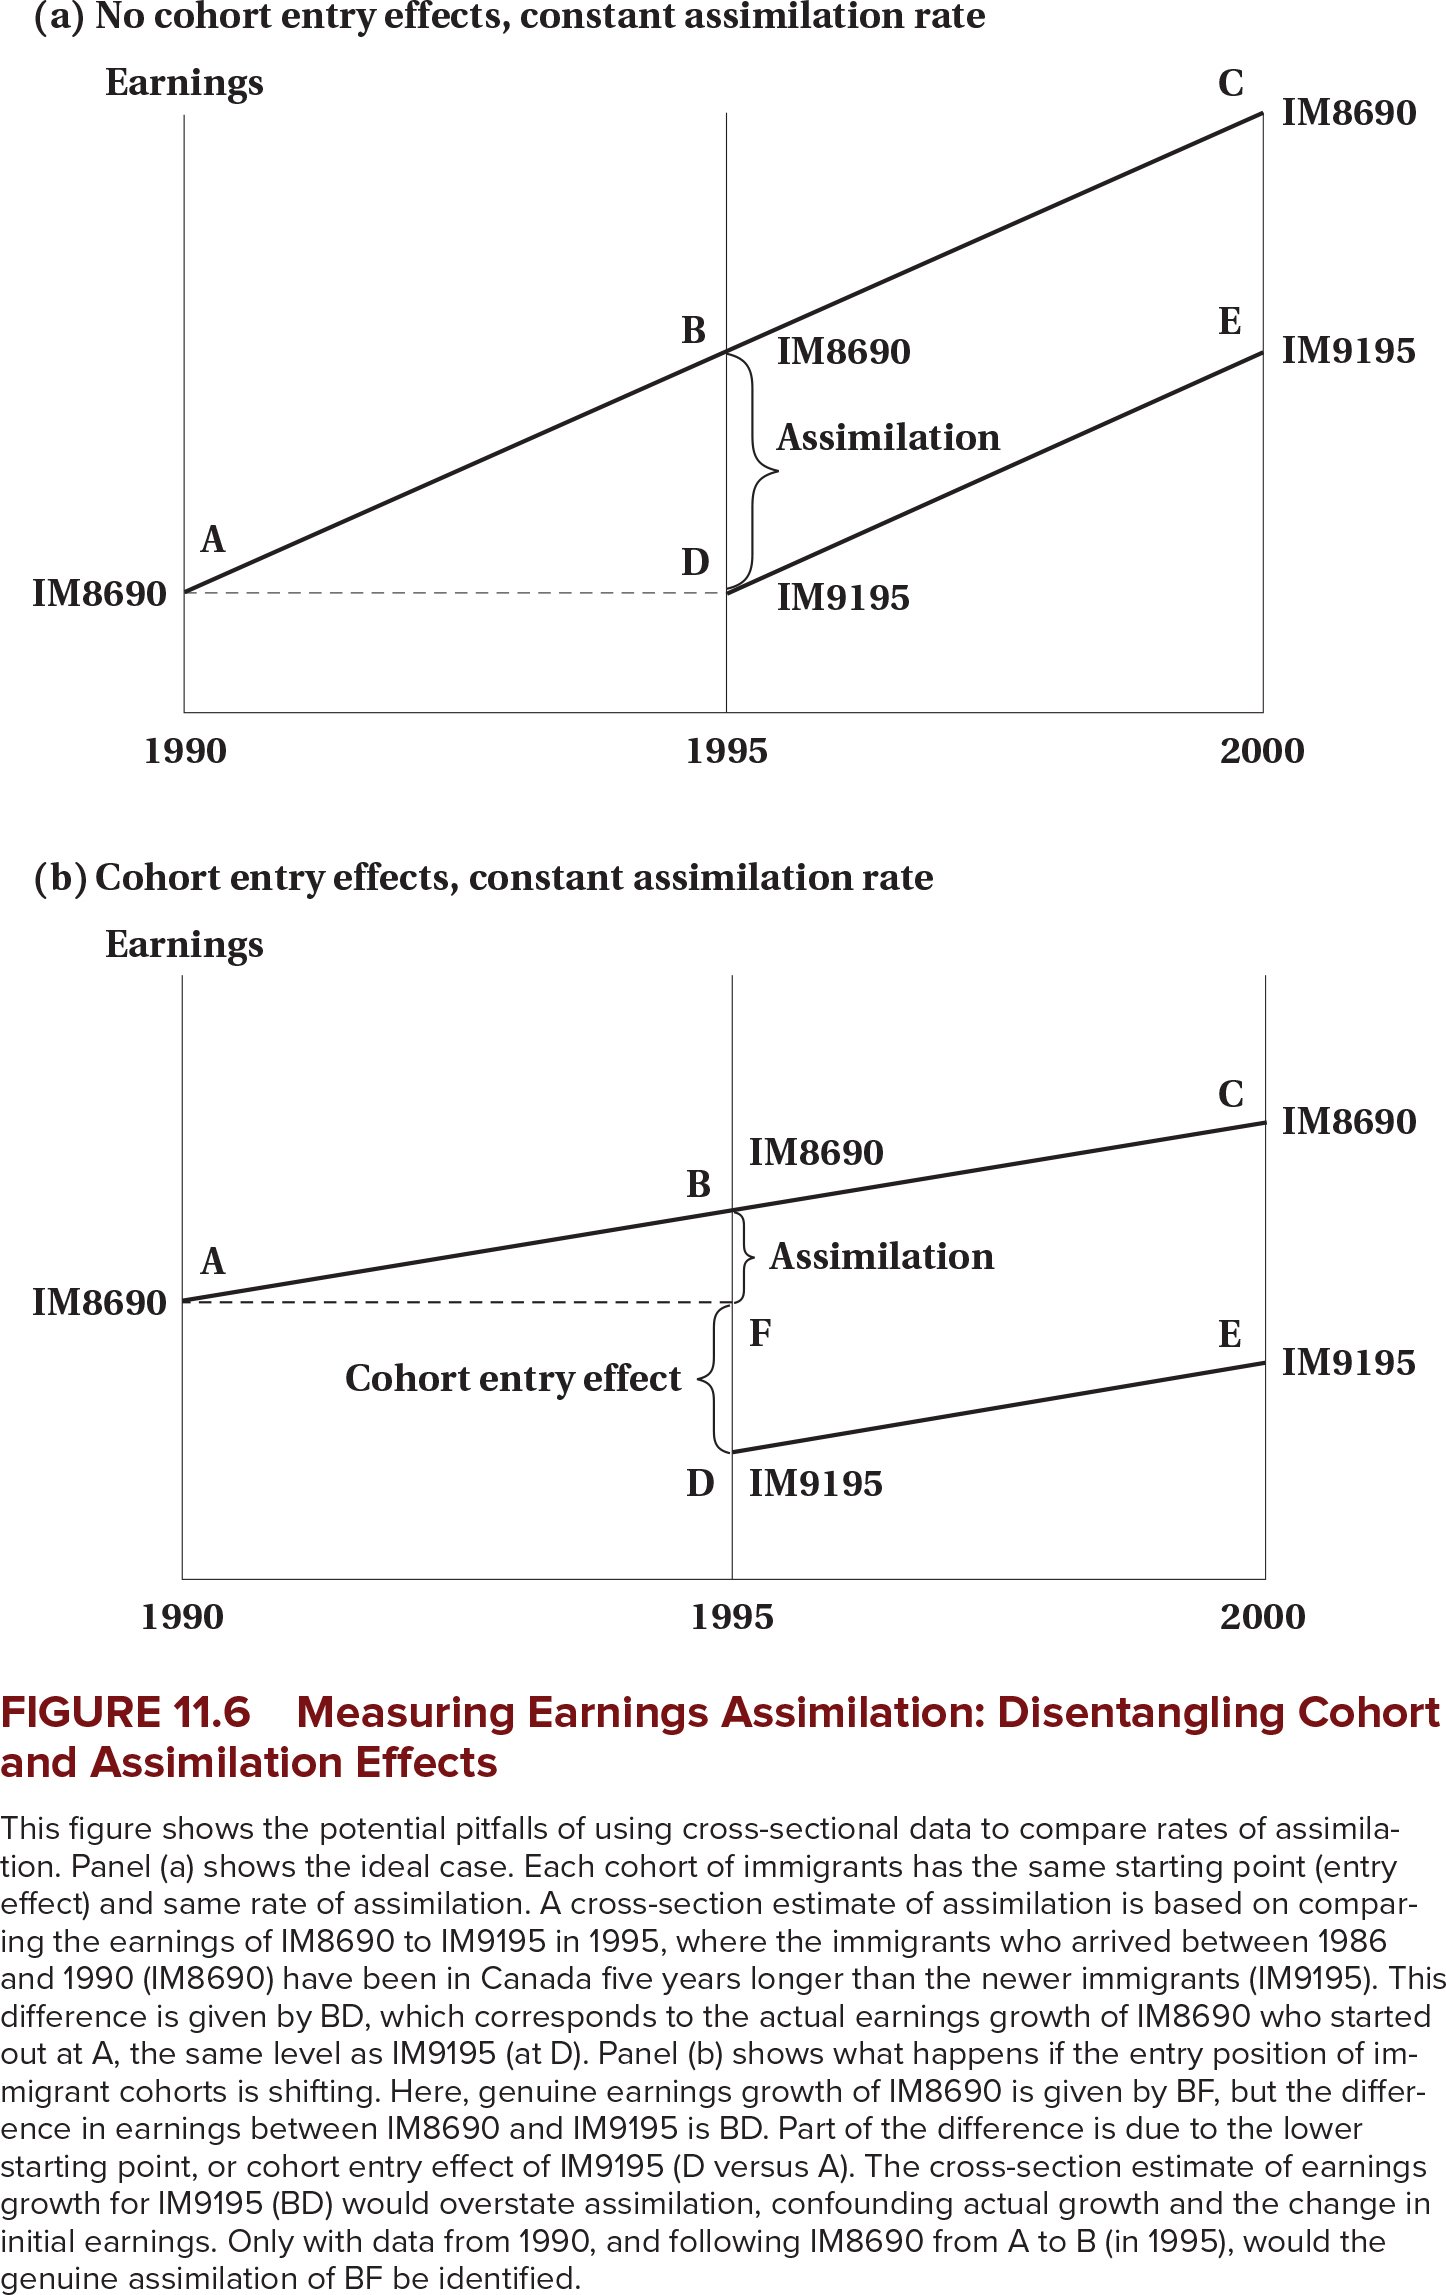
\includegraphics[width=0.43\linewidth]{ben54842_1106}
\end{frame}

\begin{frame}{Figure 11.7 -- Annual Earnings by Immigrant Cohort, 2010 and 2015 }
\centering
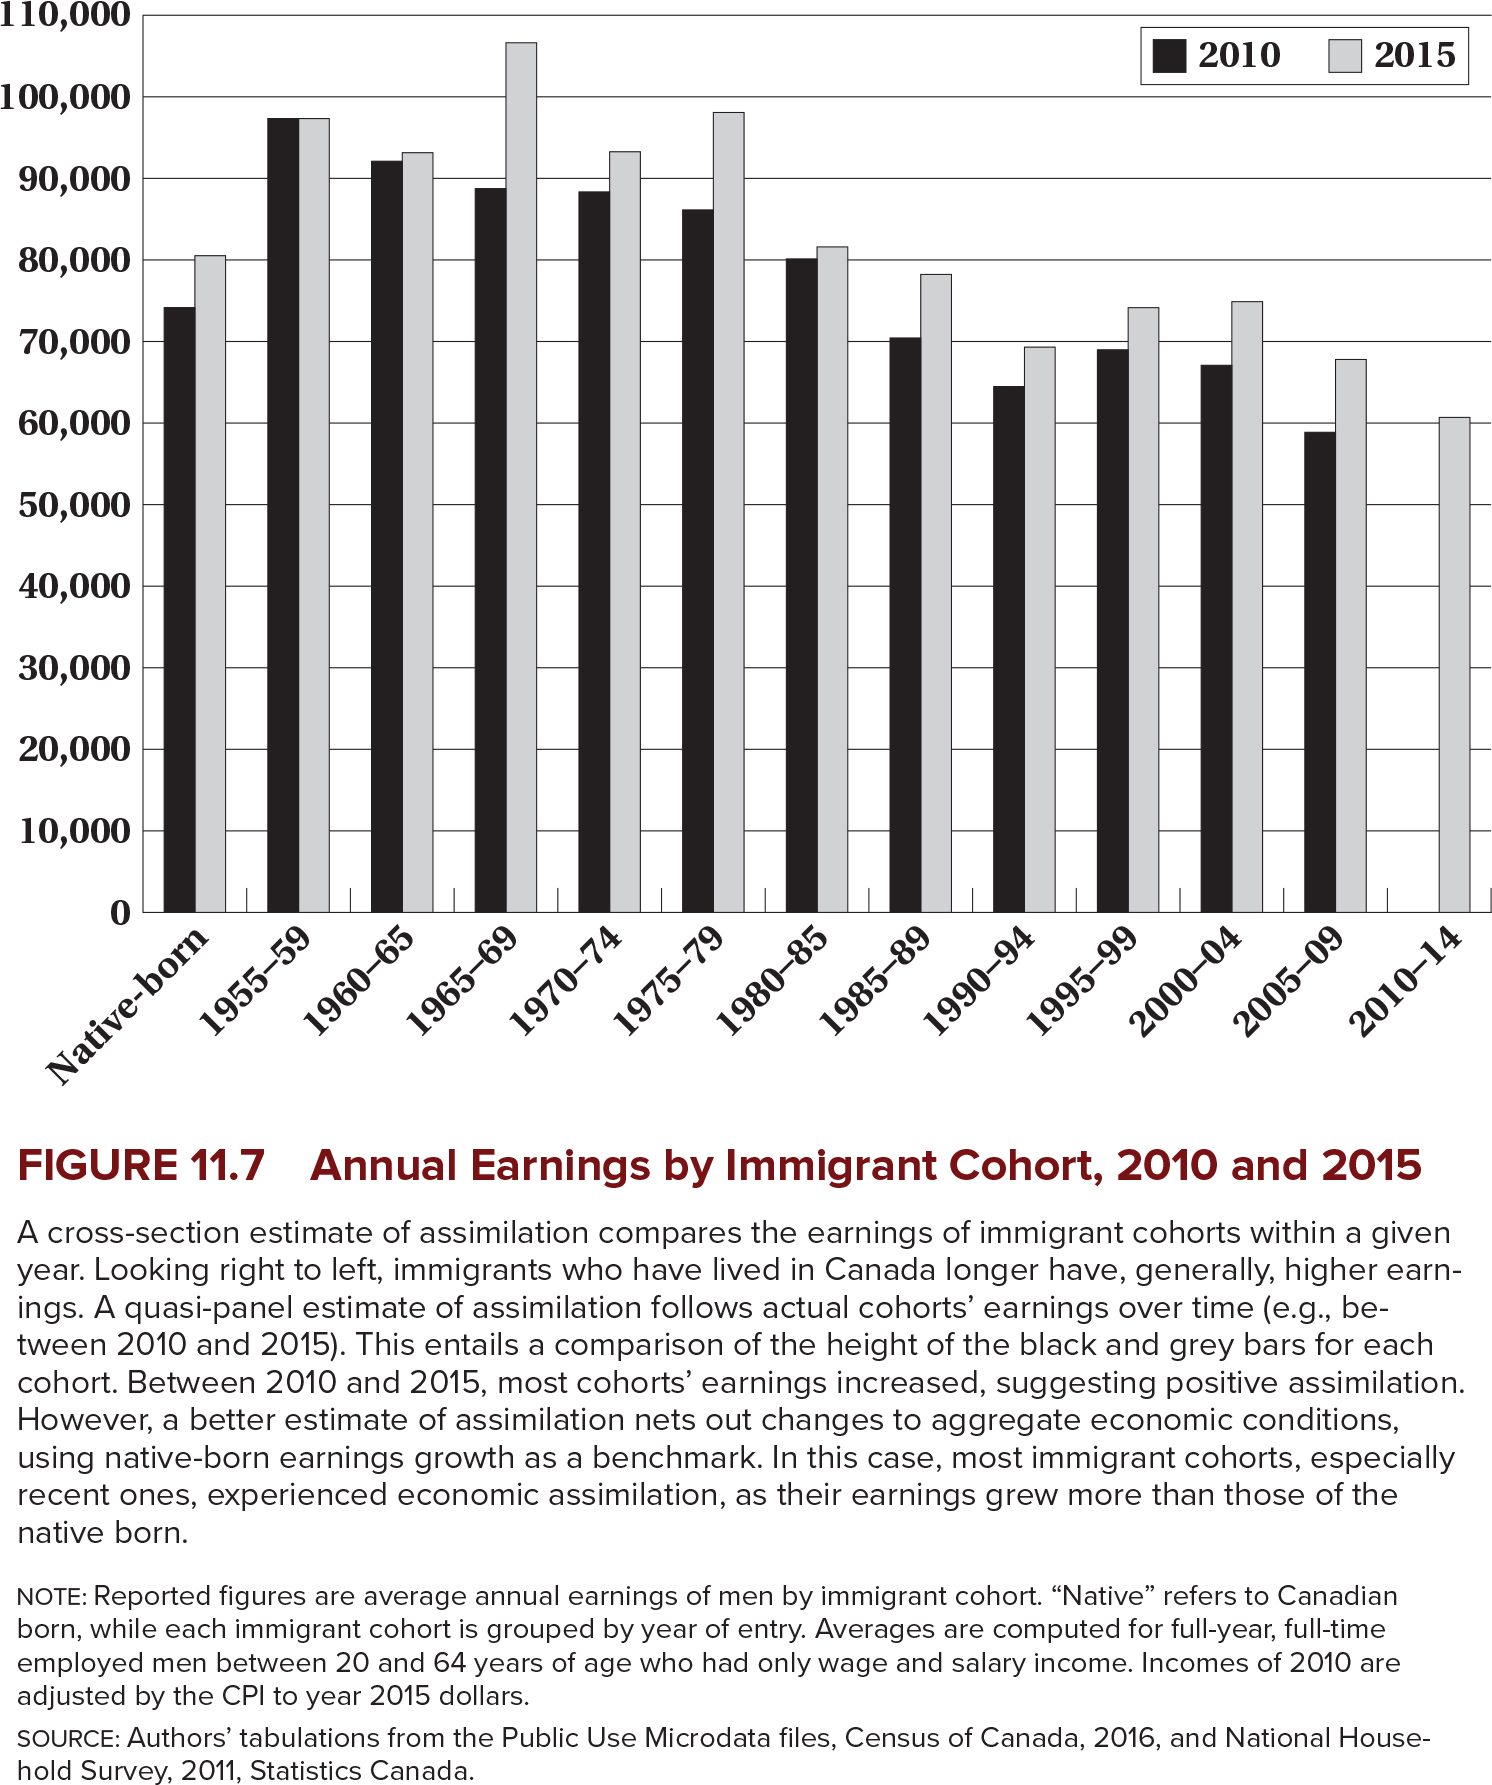
\includegraphics[width=0.67\linewidth]{ben54842_1107}
\end{frame}

\begin{frame}{Worked Example: Cross-Section vs.\ Quasi-Panel}
\transfade
\small
\begin{tabular}{lccc}
\toprule
\textbf{Cohort} & \textbf{Observed in 1995} & \textbf{Observed in 2000} & \textbf{Change 95--00} \\
\midrule
Native born & \$46{,}999 & \$48{,}641 & \$1{,}642 \\
IM8185 & \$42{,}294 & \$45{,}962 & \$3{,}669 \\
IM8690 & \$36{,}580 & \$41{,}588 & \$5{,}008 \\
IM9195 & \$31{,}423 & \$38{,}652 & \$7{,}229 \\
\bottomrule
\end{tabular}

\vspace{0.5em}
\footnotesize
\textbf{Entry effect:} Newest cohort vs.\ native born in 1995: \$46{,}999 -- \$31{,}423 = \$15{,}576.\\
\textbf{Cross-section ``assimilation'' (biased):} \$36{,}580 -- \$31{,}423 = \$5{,}157.\\
\textbf{Quasi-panel (cohort growth net of natives):} \$7{,}229 -- \$1{,}642 = \$5{,}587.
\end{frame}

\begin{frame}{Empirical Evidence on Assimilation}
\transfade
\begin{itemize}[<+->]
  \item Entry penalty has generally worsened over time.
  \item Returns to foreign education/experience are lower than to Canadian-acquired.
  \item Average cohort earnings often do not fully catch up to native-born levels.
  \item Women typically show slightly smaller entry gaps; overall patterns similar.
\end{itemize}
\end{frame}

% ============================================================
\section{Outcomes, Policy, and Source Countries}
% ============================================================

\begin{frame}{Immigrant Outcomes \& Policy Design}
\transfade
\begin{itemize}[<+->]
  \item Canada’s point system vs.\ U.S. family-reunification emphasis.
  \item Point system tilts selection toward more-skilled groups.
  \item Independent immigrants fare better on average than family/refugee classes.
\end{itemize}
\end{frame}

\begin{frame}{Impact on Source Countries: Brain Drain}
\transfade
\begin{itemize}[<+->]
  \item Less-developed countries may lose highly skilled workers.
  \item Education costs borne at home; benefits realized abroad.
  \item Policy remedies discussed in the literature (not detailed here).
\end{itemize}
\end{frame}

\begin{frame}{Worked Example: To Move or Not to Move?}
\transfade
\small
Person age 25 compares lifetime earnings (40 years).\\
Canada: \$100{,}000/year; U.S.: \$110{,}000/year; real interest \(r=5\%\).\\
\textbf{Result:} The difference in present values is \$180{,}170.41 in favour of moving.\\[0.5em]
\begin{block}{Takeaway}
Even a small annual earnings gap, compounded over a long horizon and discounted, can justify migration. Moving costs, risk, and non-monetary amenities must also be weighed.
\end{block}
\end{frame}

% ============================================================
\section{Summary}
% ============================================================

\begin{frame}{Summary}
\transfade
\begin{itemize}[<+->]
  \item Canada manages immigration via target numbers and the mix of assessed/non-assessed classes.
  \item Labour-market effects hinge on elasticities and the skill composition of inflows.
  \item Cross-sections overstate assimilation when cohorts differ; cohort tracking is essential.
  \item Policy debates include selection mechanisms, fiscal impacts, and brain drain.
\end{itemize}
\end{frame}

\begin{frame}
\centering
\Huge{\textbf{Thank You!}} \\

\end{frame}

\end{document}
